\newpage
\section{Implementationm, Central Unit module}
In this chapter it is shown the Implementation of each module, the hardware is chosen
to be compliant with the requirements of the project.

\begin{figure}[h]
	\centering
	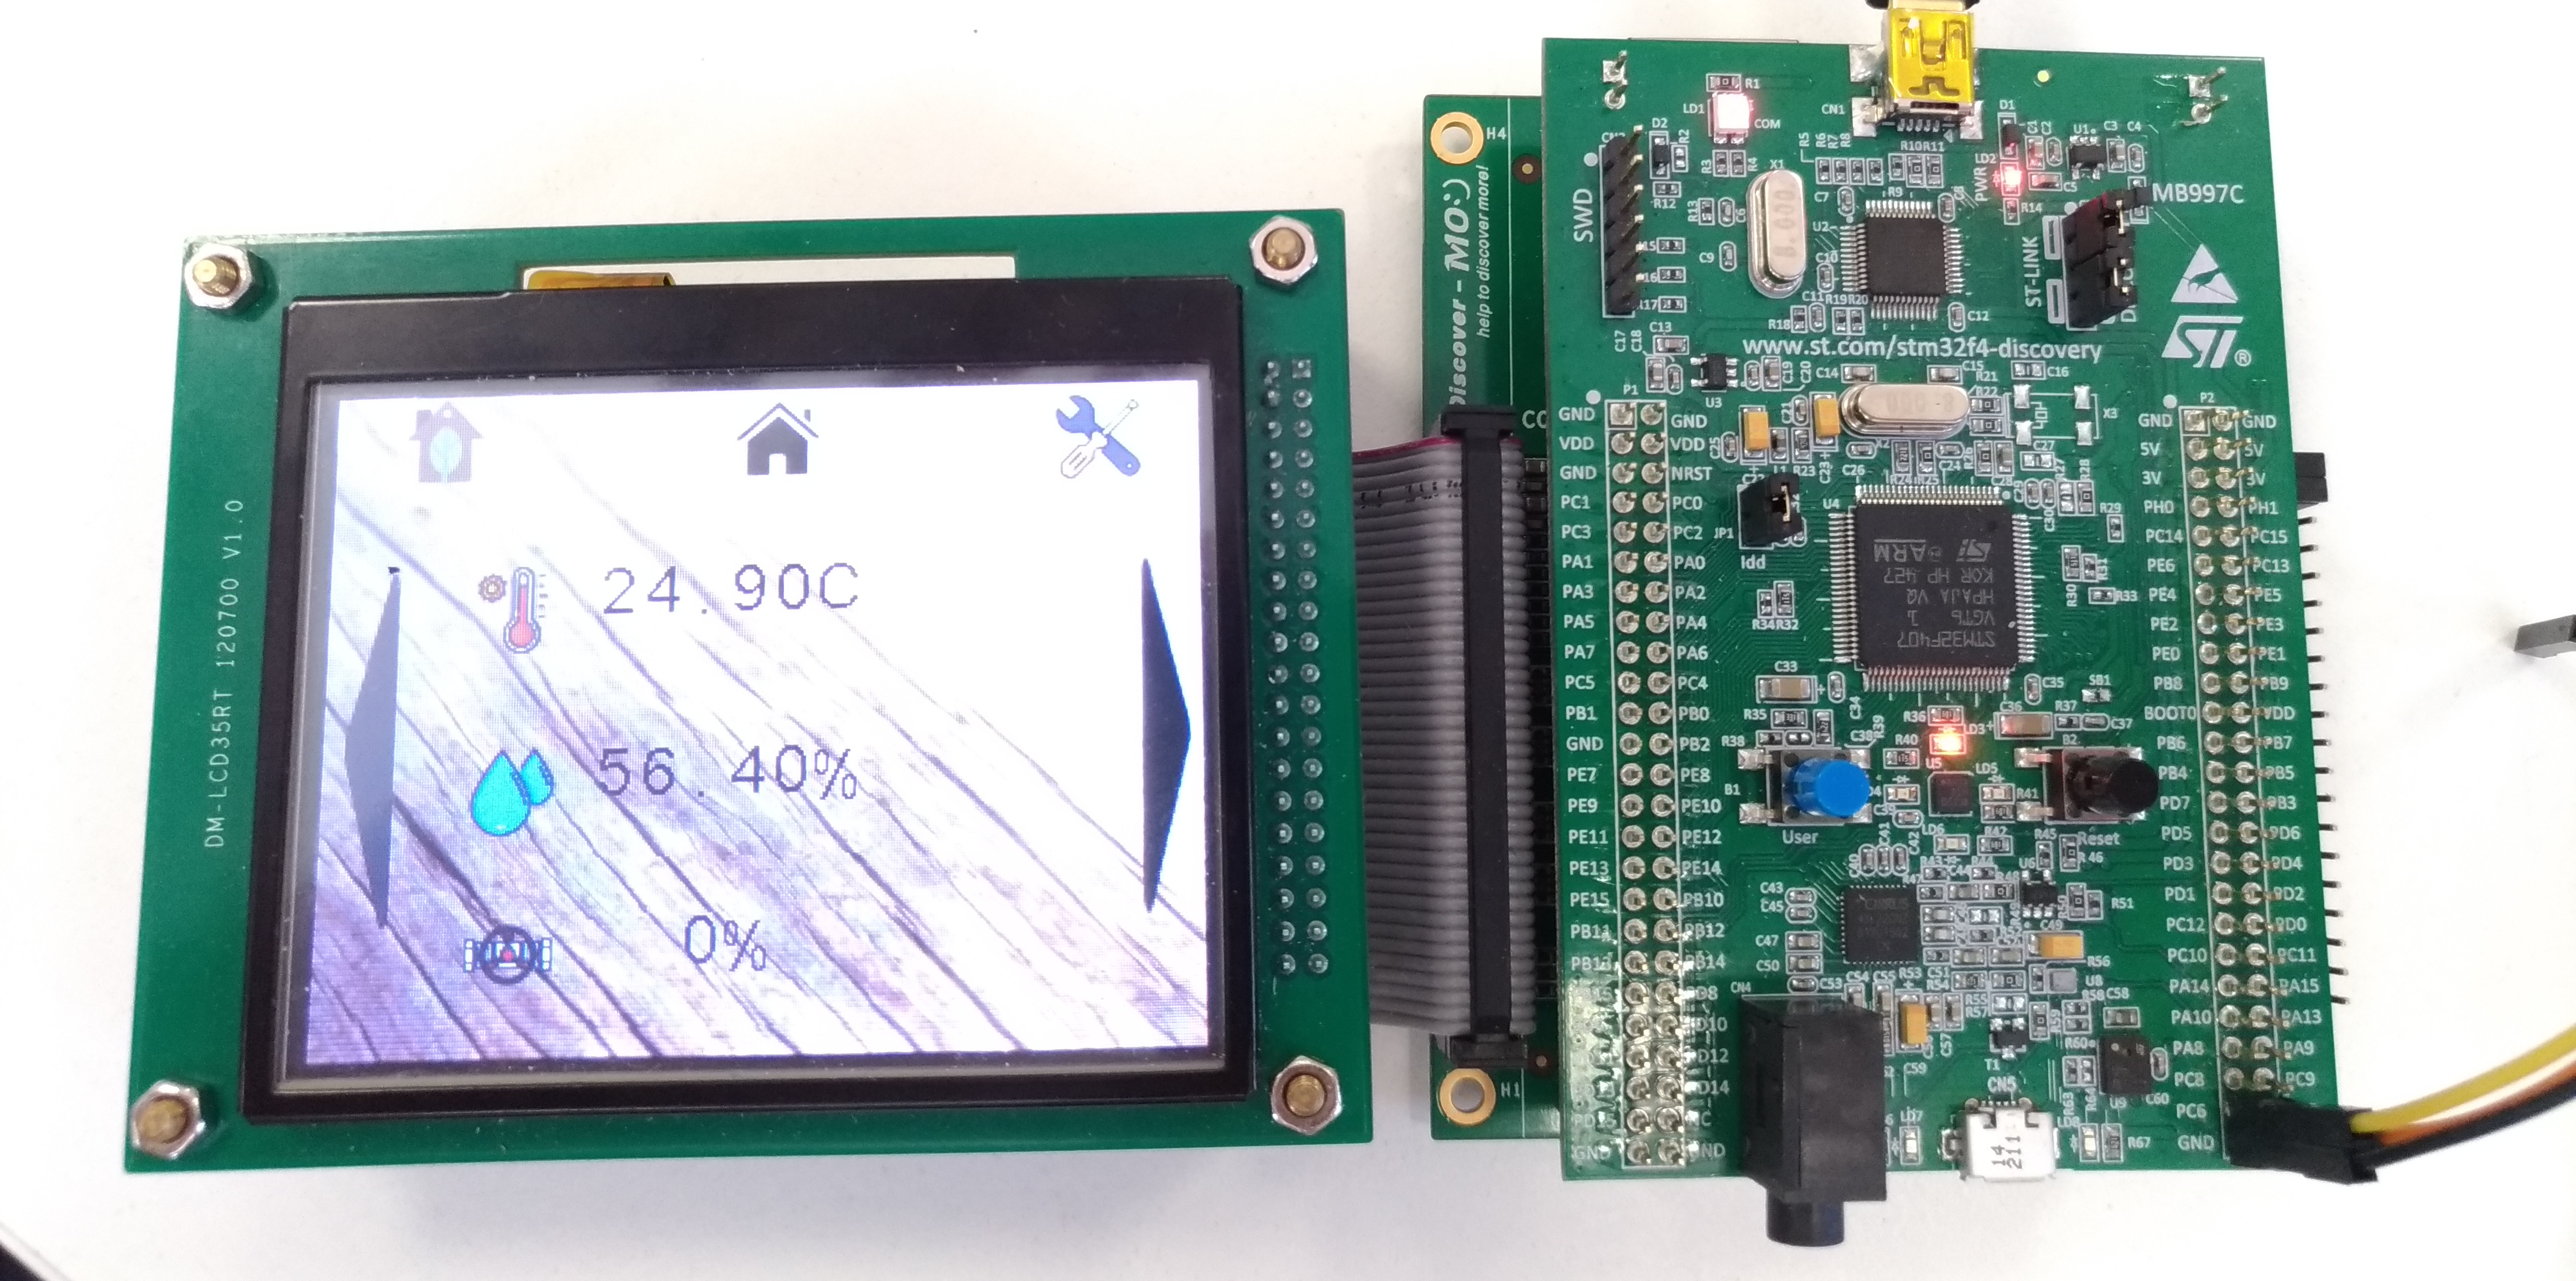
\includegraphics[width=8cm,keepaspectratio]{img/CentralUnit}
	\caption{Central Unit module}
	\label{fig:CentralUnit}
\end{figure}

The module is composed by:
\begin{itemize}
	\item STM32F407VG DISCOVERY
	\item LCD board Touchscreen 3”5
\end{itemize}


On the discovery board is running the code on top of Erika RTOS, the systen is composed by three different task:
\begin{itemize}
	\item \textbf{Graphic task} running at 10Hz (every 100ms)
	\item \textbf{Polling task} running at 0.2Hz (every 5s)
	\item \textbf{Check Message}, aperiodic task
\end{itemize}

\subsection{Wiring}

\begin{figure}[h]
	\centering
	\includegraphics[width=6cm,keepaspectratio]{img/discovery_board}
	\caption{Discovery board wiring}
	\label{fig:dicovery}
\end{figure}

The module is using the \textit{USART6} of the discovery board to comunicate with the \textit{room} module, in the following table are reported the features of the \textbf{USART6}
\begin{center}
	\begin{tabular}{||c | c | c | c | c | c | c ||} 
		\hline
		USART 	& TX pin 	& RX pin	& baud-rate & Parity Bit & Stop bits & Control Flow \\ 
		\hline
		6		&	PC6		& PC7 		& 9600 & No & 1 & No	\\ 
		\hline
	\end{tabular}
\end{center}



\subsection{Graphic Interface}
\begin{figure}[h]
	\centering
	\begin{subfigure}{0.4\textwidth} % width of left subfigure
		\includegraphics[width=4cm,keepaspectratio]{img/home_screen}
		\caption{Home screen}
		\label{fig:home_screen}
		\end{subfigure}
	\vspace{1em} % here you can insert horizontal or vertical space
	\begin{subfigure}{0.4\textwidth} % width of right subfigure
		\includegraphics[width=4cm,keepaspectratio]{img/settings_screen}
		\caption{Settings screen}
		\label{fig:settings_screen}
	\end{subfigure}
	\begin{subfigure}{0.4\textwidth} % width of right subfigure
		\includegraphics[width=4cm,keepaspectratio]{img/room_screen}
		\caption{Room screen}
		\label{fig:room_screen}
	\end{subfigure}
\end{figure}
The graphic interface is compose by three different screens:
\begin{itemize}
	\item Home screen
	\item Settings screen
	\item Room screen
\end{itemize}
The main page is the \textbf{home screen} reported in \ref{fig:home_screen}, in this page the user can see the average values of the building, 
if no room is attached it will display zero or the last computed value.
If at least one room is in \textit{room crashed mode} then a warning appear on the home screen.
If at least one room is in \textit{eco mode} then an \textit{eco} icon is displayed on the home screen.
Depending on the difference between the desired temperature and the actual average temperature the termometer icon will change in cold or hot.
In the \textbf{settings screen} reported in \ref{fig:settings_screen} it is possible to set the desired temperature of the building.
In the \textbf{room screen} reported in \ref{fig:room_screen} is displayed the status of the selected room, status composed by:
\begin{itemize}
	\item Eco mode
	\item Temperature
	\item Humidity
	\item Valve position
\end{itemize}
